\documentclass[../rzero]{subfiles}
\begin{document}
\chapter{Electromagnetism}\label{electromagnetismChapter}

\begin{chapquote}{Eric Weinstein talking to Brian Keating, \textit{Youtube\cite{drbriankeatingEricWeinsteinTheoretical2020}}}
``You guys need more money. You struck the worlds worst licening deal.''
\end{chapquote}


\section{What is Electromagnetism}
Essentially, it's light and electricity. Beams of light move at the speed of light, and electrons and other particles carry charge. 

\section{Electromagnetism from General Relativity}
Here is the part where I get to do the physics equivalent of pulling a rabbit out of a hat. Everyone \textit{knows} that since electromagnetism is so much stronger than gravity, my task here is not merely hopeless. So let's see just how funny we can get here. 



\section{Starting}
The emergence of electromagnetic phenomena from General Relativity comes from starting at an electron model. Since an electron is a spinning thing, with known mass and angular momentum, I start with the known General Relativity solution for a spinning thing with mass, the  solution found in 1963 by Roy Kerr\cite{kerrGravitationalFieldSpinning1963}. I don't use the Kerr - Newman 'charged' solution\cite{newmanNoteKerrSpinningParticle1965}, after all I am attempting to get electromagnetism to emerge from General Relativity, so I can't just toss electrical stuff in there at the outset, right? Burinskii\cite{Burinskii2008} and others have employed Kerr Newman solutions as possible models for the electron, but, as I stated, I'm not using built in charge. I am attempting to construct charge from gravtitational phenomena.

The Kerr solution for a particle of the same mass and spin as an electron is known in the biz as a 'naked singularity', which is a thing that 99$\frac{99}{100}$\% of physicists think can't exist, but they won't argue that it is a solution of Einsteins vacuum equations from equation (\ref{vacuumEquation}). So yes, we are going to have to throw caution to the wind here and just assume that the Kerr solution (or something like it as we will see in chapter \ref{electronModelChapter}) is a reasonable model of the electron. 

As a defence of my so far nascnet electron model, I will point out that there is no truly self consistent model of the electron known at this point. As the Richard Feynman one of a few authors of QED, our best 'standard physics' model of the electron pointed out\cite{Feynman1985} (page 127): 

\begin{quotation}
"The shell game that we play to find n and j is technically called “renormalization.” But no matter how clever the word, it is what I would call a dippy process! Having to resort to such hocus-pocus has prevented us from proving that the theory of quantum electrodynamics is mathematically self-consistent. It’s surprising that the theory still hasn’t been proved self-consistent one way or the other by now; I suspect that renormalization is not mathematically legitimate." 
\end{quotation}

A typical physics professor will tell you that renormalization isn't a problem - and they are right - but only because so many worse problems have arisen in theoretical physics over the past 7 decades since QED, so that QED renormalization now seems like a walk in the park. To be fair, it does actually work. (Although see Consa\cite{Cioletti2006} for a negative outlook on the QED industry.)

Basically, the problem in all electron models, including QED, is quite simple to elucidate: the electron explodes when you try to assemble a model from charge - the energy you need to bring together 'bits of a charge' to form a small thing that looks like an electron goes to infinity. The problem is that charge is modelled as a 'charged goo' and each bit repels all the other bits as you try and squeeze it all into one place. I'll go into this more in chapter \ref{physicsTodayChapter}.  

This Kerr naked singularity turns out to be very long (some $num{1e42}$ longer than the natural size of the electron). Conceptually dividing this long singularity into  $num{1e42}$ sections, I find that each section has a gravitational wave interaction about equal to the gravitational Newtonian interaction between two electrons. And all these small interactions add up to a huge Coulomb level force between two of them.  

\subsection{How to add it up}
The expression for the electromagnetic Coulomb force $F_e$ between two electrons is 

\begin{equation}\label{coulomb_force}
	F_e = k_e\frac{q^2}{r^2} = \pm \frac{\alpha \hbar c}{r^2}.
\end{equation}

The second version is for single point charges only. It is a more fundamental way of looking at electrostatics, since in reality all charges are of unit size. I will use this second one. Note that:

\begin{itemize}
  \item $\alpha$ is a number, about 1/137.\footnote{Feynman - "all good theoretical physicists put this number up on their wall and worry about it." (I doubt they do any longer --tom) }
  \item $\hbar$ is the famous quantum constant.
  \item $c$ is the speed of light.
  \item $r$ is the distance between the two electrons.
\end{itemize}

For for the force of gravity $F_g$ we have

\begin{equation} \label{grav_force}
	F_g = G\frac{m_e^2}{r^2}.
\end{equation}

Where

\begin{itemize}
  \item $G$ is Newton's gravitational constant.
  \item $m_e$ is the mass of the electron.
  \item $r$ is the distance between the two electrons.
\end{itemize}

The large, famous value of the ratio between these two forces, which I will call $k'$ is by inspection of eqn (\ref{coulomb_force}) and (\ref{grav_force})

\begin{equation} \label{electric_ratio}
	k' = ratio_{electric} = \frac{k_e q_e^2}{G m_e^2} = \frac{\alpha \hbar c}{G m_e^2} = \num{4.166e42}
\end{equation}


I will now construct a force $k'$ stronger than the usual Newtonian gravitational force using only the Kerr solution of Einsteins equations, with no reference to electromagnetism. If your afraid of magicians, look away, now.

\section{The Kerr Singularity with Electron Parameters}
The well known Kerr solution of Einsteins equations has a naked ring singularity for $J/mc > Gm/c^2$, somewhat better known as $a > m$ in geometric units. I use SI units in this section. In Kerr-Schild coordinates (a coordinate system that is Minkowskian almost everywhere)\cite{Visser2008}, the expression for the location of the ring singularity is $x^2 + y^2 = (J/mc)^2$, (avoiding the use of r, as r has a meaning on its own in the Kerr solution in Kerr-Schild coordinates). Using the measured experimental values for the mass $m_e$ and spin angular momentum $\hbar/2$ of an electron, the radius of the ring singularity is:
\begin{equation} \label{radius_eqn}
	R_{ring} = J/mc = \hbar/2m_ec = \num{1.93e-13}m
\end{equation}

Thus the ring singularity is 0.5 of the Compton wavelength in circumference. This is a \textit{huge} radius, and I will go into how this sort of thing might be possible in chapter \ref{electronModelChapter}. This radius can also be calculated as a ratio. The obvious other gravitational length to compare it to is the Schwarzschild radius $r_s = 2Gm_e/c^2$ for the electron mass:

\begin{equation}
	size \ ratio = \frac{\hbar/(2m_ec)}{(2Gm_e/c^2)} = \frac{\hbar c}{4G m_e^2} = \num{1.4e44}
\end{equation}

 It is noteworthy that this ratio is already very close to the ratio $k'$ of the strength of the electric Coulomb force to the gravitational attraction between two electrons. Indeed, multiplying this ratio by the four times the fine structure constant (i.e. $\approx 0.029 $ ) gives one \textit{exactly} $k'$ - the ratio of the electric and gravitational force on two electrons.
 
\begin{equation}
	ratio = 4\alpha \frac{\hbar/(2m_ec)}{(2Gm_e/c^2)} = \frac{\alpha \hbar c}{G m_e^2} = \num{4.166e42} = k'
\end{equation}


These are of course the same arrangement of constants as in (\ref{electric_ratio}). The difference here is that this ratio is now calculated without any references to the electric Coulomb force. It is simply a ratio of the radius of a Kerr singularity of the electron's mass and spin angular momentum to that of Schwarzschild radius for the electron mass $r_s$, along with a factor of $4\alpha$ added in by hand (see the next section). 

Things are getting interesting, but we're not there yet. What we have is a ring that measures $\num{1.4e44}$ times the size of an un-spinning black hole the mass of an electron. The next question is how do two of these rings a distance $r$ apart interact strongly?


\section{Gravitational Waves as carriers}

%There is a connection between the size of the Kerr ring singularity as measured in units of the electron Schwarzschild radii($r_s$) to the effect of Coulomb repulsion. Can charge itself be constructed of nothing more than geometry? The mere calculation of the ratio does not give one a recipe for how electromagnetism can be constructed from general relativity, but there are some hints at a mechanism.
\begin{figure}\label{kerr-electric-image}
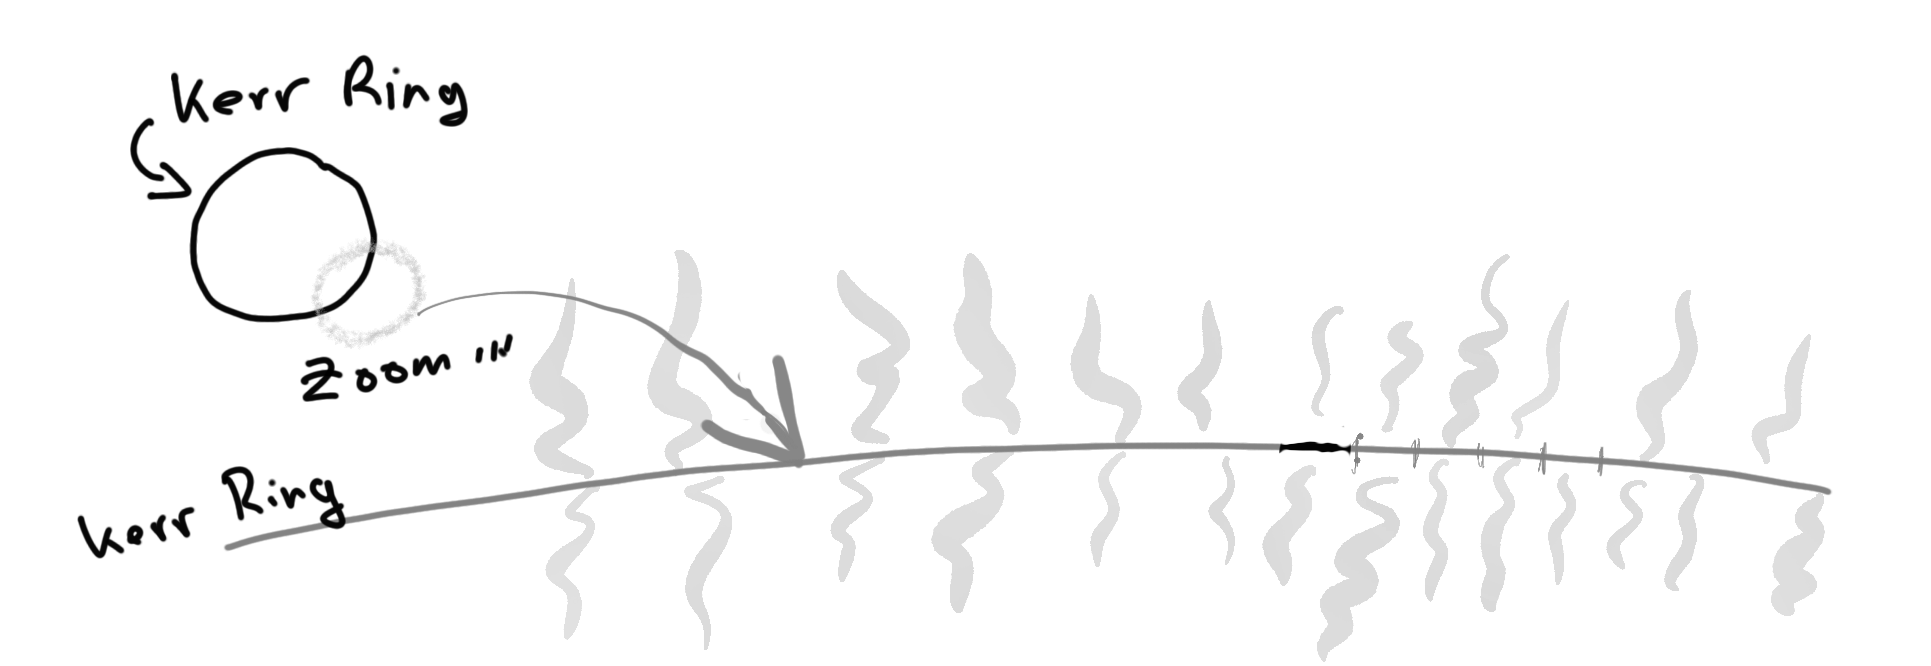
\includegraphics[width=0.99\textwidth]{chapters/images/kerr-electric.png}
\caption{Upper left: A Kerr ring singularity. Main: zoom in on a small section of it to reveal gravitational waves of a wavelength equal to the Schwarzschild radius (and up). This results in about $\num{1.4e44}$ segments, each interacting with an $\alpha$ cross section.}
\end{figure}



 If one imagines the ring singularity is cut into $\num{1.4e44} $ pieces each of size $r_s$ and each piece interacts with the nearby electron with a 'gravitationally sized' force on each section of $\alpha G m_e^2/r^2 $, perhaps one can create electromagnetic strength forces from entirely gravitational means. $4\alpha$ then is perhaps some scale factor/antenna cross section of 'order 1' (well $ 0.029$).
   
 How can a single section of the ring with a tiny mass of $ 10^{-44}m_e $ and length $r_s$ interact so strongly? The answer must lie in gravitational wave interaction. That's all I really have since the point of this book is to build physics with nothing but General Relativity.  It seems that the properties of a singularity are such that it should interact very well\cite{Nakamura1993} with gravitational waves. A gravitational wave effect could thus be strong enough to provide a net force of $\alpha G m_e^2/r^2 $ per segment, with super radiance and absorption taken into account. For comparison, an astrophysical black hole of radius $r_s$ can emit or absorb a significant (~10\%!) of its energy given the right gravitational wave parameters.\cite{Brito2015}.  
  
 Each section would need to be interacting with gravitational waves of a fantastic frequency - the wavelength would have to match the Schwarzschild radius ($r_s$) of the electron. This is of course a frequency well beyond that usually conceived in accepted quantum physics - but remember - I am trying to also emerge quantum mechanics from General Relativity, so I'm asking you to sit on this 'annoyance' for a while (until chapter \ref{quantumMechanicsChapter}).  In for a penny and all that.
 
 The amplitude of the gravitational waves at this incredible, $\num{2e65} Hz$ frequency is tiny, much too small to cause measurable 'gravitational' effects - we would only see the force of one electron on another as they exchange gravitational wave energy. These waves are of many orders of magnitude smaller in amplitude than those measured by LIGO, for example.
 
 Once we have individual segments interacting with a the right force we have recreated the Coulomb force, or at least a rough mechanism as to how it would work. Another way of thinking of it is to look at the overall energy balance - the waves configuration of two electrons will drop in energy as the two electrons move further apart from each other. Cetto\cite{Cetto2013} outlines a physical description of QED, one that uses a more physical model of QED. 
  
 An electron model based on a Kerr ring has some references in the literature - see for example Burinski\cite{Burinskii2012}. The more general model of an electron as a ring of some sort (or a particle on a ring) of Compton radius is discussed mostly in respect to the zitterbewegung motion from the Dirac equation. See Hestenes\cite{Hestenes1990}, Maddox\cite{Maddox1987}, and Barut\cite{Barut1984}.
 
 \section{Electromagnetism - non Coulomb interactions} 
 Essentially, electromagneitic waves - photons are constructed as modulations of these fundamental gravitational waves - the gravitational waves are carrier waves. In this model, spin 1 is simply a result of moving a charge up and down. 
 
 If you think you know that spin 1 photons can't be built with spin - 2 gravtiational waves, I have news for you. Here, for instance is someone\cite{shiObservationAcousticSpin2019} building spin 1 from a scalar (pressure wave) acoustic field. Basically, you get spin 1 by taking a source exchanging energy and wiggling it up and down. Another source/receptor will see the other source and vibrate up and down in the same direction. The experimentally observed spin of a field can be emergent. As an example Cetto de la Peña obtain fermion statistics from a spin one field.\cite{cettoElectronSystemCorrelated2016}. Here Barceló\cite{barceloElectromagnetismEmergentPhenomenon2014} shows how one might emerge electromagnetism itself. Also see Ranada\cite{ranadaTopologicalTheoryElectromagnetic1989}.
 
 The idea is to use this fundamental energy exchange via gravitational waves as a carrier wave for electromagnetic waves. An EM wave is thus composed of trillions of trillions of gravitational carriers - underneath it, so to speak. 
 
 I am going to need to expand this, get some drawings going, etc. 
  
  Lorentz + Coloumb == EM. 

 \section{Calculating \texorpdfstring{$ \alpha $}{Alpha}} 
 The hypothesis that these ultra high gravitational waves 

\section{Discussion}
While there are of course other more pedestrian explanations, this ratio result is exact - it is not approximate numerology.

The interpretation section above postulated gravitational wave interactions between Kerr solutions with electron mass and angular momentum parameters as a mechanism to start to build electromagnetism from general relativity. Irrespective of any validity to those guesses it's \textit{still} a mystery as to why the scale of the Coulomb force to the gravitational force is identical with the radius of the Kerr ring singularity to the much smaller Schwarzschild radius of an electron mass.

Indeed, this Kerr - Coulomb ratio is interesting in its own right, even if a direct physical interpretation is not imagined. Wheeler's Geometrodynamics \cite{Wheeler1957a} seeks an already unified picture, but Wheeler in no way hypothesizes that EM can emerge from gravitation. 


\end{document}
